\documentclass[
  ngerman,
  DIV=14
]{scrartcl}
\usepackage{babel}
\usepackage{csquotes}

% typography
\usepackage{fontspec}
%\usepackage[utopia]{mathdesign}
\usepackage{newpxmath}
\setsansfont{Open Sans}[
  BoldFont={Open Sans Bold},
  ItalicFont={Open Sans Italic}]
\setmonofont[Scale=0.87]{Menlo}
\setmainfont{Palatino}
\linespread{1.15}
%\renewcommand\familydefault{\sfdefault}
\usepackage[factor=1000]{microtype}

% graphics, drawings, etc.
\usepackage{xcolor}
\usepackage{graphicx}
\usepackage{tikz}
\usetikzlibrary{shapes.geometric}
\usetikzlibrary{shapes.arrows}
\usetikzlibrary{positioning}
\usepackage{pgfgantt}

% highlighting, lists, code
\usepackage{listings}
\usepackage{booktabs}
\usepackage{soul}
\lstset{
  basicstyle=\ttfamily,
  %escapeinside=||,
  keywordstyle=\color{blue!50!black},
  stringstyle=\color{green!50!black}}
\capsdef{////}{\sffamily\bfseries\scshape}{.10em}{.4em}{.2em}
\newcommand{\tablespacing}[1]{\renewcommand{\arraystretch}{#1}}

% math
\usepackage{amsmath}
\usepackage{siunitx}

% links
\usepackage[
  colorlinks,
  linkcolor={red!50!black},
  citecolor={blue!50!black},
  urlcolor={blue!80!black}
]{hyperref}

\subject{Software Engineering}
\title{Übung 2: Projektplanung}
\subtitle{Lösung}
\author{Patrick Elsen}
\date{Wintersemester 2018-2019}
\publishers{Technische Universität Darmstadt}

\begin{document}
\maketitle

\section*{Problem 1: Klassifizierung}

\emph{Geben Sie für die folgenden Anforderungen an, ob es sich um funktionale oder nicht-funktionale Anforderungen handelt. Geben Sie außerdem an, ob es sich um Nutzer- oder Systemanforderungen handelt. Begründen Sie Ihre Klassifizierung kurz.}

\begin{table}[!h]\centering\tablespacing{1.3}
\begin{tabular}{@{}p{4.5cm}p{4cm}p{6cm}@{}}
\toprule
\caps{ANFORDERUNG} & \caps{FUNKTIONAL} & \caps{USER OD. SYSTEM}\\
\midrule
\emph{Die Webseite muss in allen gängigen Browsern korrekt angezeigt werden.} & Nein, dies ist eine Anforderung an die Benutzbarkeit des Systems. & Benutzeranforderung, weil hier in natürlicher Sprache eine Bedingung des Systems spezifiert wird.\\
\emph{Nutzer können Routendateien hochladen um Routen darstellen zu können.} & Ja, dies ist eine klare Funktionalität. & Systemanforderung, weil hier in natürlicher Sprache ein Dienst des Systems beschrieben wird.\\
\emph{Die Import-Funktion darf, unabhängig von der Größe der Eingabedatei, nicht mehr als 100 MB RAM allozieren.} & Ja, dies ist eine klare explizite Funktionalität. & Systemanforderung, da hier eine Beschränkung explizit festgelegt wird (100 MB RAM).\\
\emph{Die Zeit bis zur Darstellung der Webseite darf 150 ms nicht überschreiten.} & Nein, dies ist eine Qualitätsanforderung (Performanz). & Systemanforderung, da hier eine Beschränkung explizit festgesetzt wird.\\
\bottomrule  
\end{tabular}
\end{table}

\section*{Problem 2: Überprüfbarkeit}

\emph{Bewerten Sie, ob die folgenden nicht-funktionalen Anforderungen geeignet sind, um ihre Erfüllung überprüfen zu können. Wenn eine Anforderung nicht erfüllbar ist, geben Sie eine verbesserte Formulierung an, die die Überprüfbarkeit sicherstellt.}

\medskip\noindent
\emph{Es darf nicht möglich sein, Kommentare mit beleidigendem Inhalt zu veröffentlichen.}

\medskip\noindent
Was ist denn beleidigend? Für wen ist es beleidigend? Beispiel: Die meisten Menschen in Deutschland würden zustimmen, dass das Wort \enquote{Hurenkind} beleidigend ist und keinen sinnvollen Verwendungszweck in der Kommunikation hat. Typographen bezeichnen mit \emph{Hurenkind} jedoch eine einzelne Zeile eines Absatzes, die vom Rest des Absatzes getrennt auf einer neuen Seite steht (dies ist generell zu vermeiden). Ebenso schwierig ist es, wenn man sich mit religiösen Zuständen befasst, denn was für den einen eine freie Meinungsäußerung ist, kann der andere als beleidigend auffassen, und das endet geschichtlich gesehen oft in Mord, Todschlag oder Hexenverbrennung.

\bigskip\noindent
\emph{Der Quellcode muss die Java Coding Conventions einhalten.}

\medskip\noindent
Dies ist eine überprüfbare Anforderung. Die Java Coding Convention ist ausreichend spezifiziert, um diese sogar mechanisch mit einem kleinen Programm wie \texttt{checkstyle} anzuwenden und zu überprüfen. Modernere Programmiersprachen haben sogar mittlerweile Programme, die den Programmierstil nicht nur automatisch überprüfen, sondern auch reparieren können (z.B. \texttt{clang-for\-mat}, \texttt{rustfmt}).

\bigskip\noindent
\emph{Die Anwendung muss unter Arch Linux lauffähig sein.}

\medskip\noindent
Dies ist halbwegs eine überprüfbare Anforderung. Man kann sehr leicht testen, ob die Anwendung unter Arch Linux funktioniert. Das einzige Manko hier ist, dass keine Version von Arch Linux angegeben wurde (was auch nicht unbedingt sinnvoll wäre, da Arch keine Versionierung besitzt). Besser wäre es, wenn man das festlegt.

\bigskip\noindent
\emph{Die Benutzeroberfläche zur Routenplanung muss intuitiv benutzbar sein.}

\medskip\noindent
Intuition ist keine messbare Größe. Besser wäre es, wenn man bestimmte Metriken festlegt und kontrolliert. Zum Beispiel könnte man die Anzahl an Falschbedienungen messen, und dafür sorgten, dass diese weniger als 1\% der Gesamtinteraktionen ausmachen.

\section*{Problem 3: Formulierung nicht-funktionaler Anforderungen}

\emph{Die Erfüllung der folgenden nicht-funktionalen Anforderungen ist in dieser Form nicht überprüfbar. Recherchieren Sie geeignete Kriterien, anhand derer die Anforderungen überprüft werden können. Geben Sie eine neue Formulierung der Anforderungen an, die anhand dieser Kriterien überprüfbar ist. Nennen Sie auch die Quellen, auf die Sie sich stützen!}

\medskip\noindent
\emph{Benutzern einer VR-Brille dürfen durch die Anwendung keine Kopfschmerzen oder Schwindel entstehen.}

\medskip\noindent
Laut einer Stude können bis zu 61\% der Menschen von VR-Technologie (temporäre gesundheitliche Probleme entwickeln\footnote{\url{https://www.ncbi.nlm.nih.gov/pubmed/8074626}}. Deswegen geben Hersteller von VR-Equipment Sicherheitshinweise\footnote{\url{https://www.oculus.com/legal/health-and-safety-warnings/}} aus, die sich auf diese Probleme beziehen. Wenn man vermeiden möchte, dass Menschen Kopfschmerzen oder Schwindel bekommen, muss man zuerst verstehen, wodurch diese Symptome ausgelöst werden, und dann gezielt darauf Anforderungen setzen.

\bigskip\noindent
\emph{Die Benutzeroberfläche der Applikation muss auf den allermeisten aktuellen Smartphones benutzbar sein.}

\medskip\noindent
Gartner, eine Britisches Consultingunternehmen, hat 2017 Statistiken zu Smartphoneproduzenten\footnote{\url{http://www.gartner.com/newsroom/id/2665715}} veröffentlicht. Danach sind Samsung, Apple und Huawei die drei weltweit größten Produzenten nach der Anzahl an verkauften Smartphones. Laut Wikipedia waren 2016 die meistverkauften Smartphones das Apple iPhone 7 mit 50,8 Millionen verkauften, das Samsung Galaxy S7 mit 55 Millionen verkauften Einheiten, sowie das Redmi note 3, das OnePlus 3t, das Redmi 3s prime und das Lenovo K4 note\footnote{\url{https://en.wikipedia.org/wiki/List_of_best-selling_mobile_phones}}. Es würde also Sinn ergeben, wenn man angibt, dass die Benutzeroberfläche auf diesen nutzbar sein soll.

\bigskip\noindent
\emph{Die von der App mit Emojis dargestellten Emotionen sollen unabhängig vom Kulturkreis verständlich sein.}

\medskip\noindent
Kulturkreise unterscheiden sich in oft unvorhersehbaren Weisen. Es würde sehr wenig Sinn ergeben, alle potenziellen Kulturkreise zu untersuchen auf deren Interpretation der Symbolik, die durch Emojis gegeben ist. Besser wäre es, anderen Kulturkreisen Emojis beizubringen. Dies würde wahrscheinlich gut klappen, denn historisch gesehen sind Emojis ja eine japanische Erfindung, die durch Apple in den Westen exportiert wurde. Damals musste man noch eine japanische Tastatur aktivieren, um diese schreiben zu können. 2010 hatten Apple und Google es geschafft, Emojis in den Unicode-Standard einzubauen, was es auch anderen Geräten ermöglichte, Emojis zu unterstützen, wie in Abbildung \ref{fig:emojis} zu sehen ist.

\begin{figure}[!t]
\centering
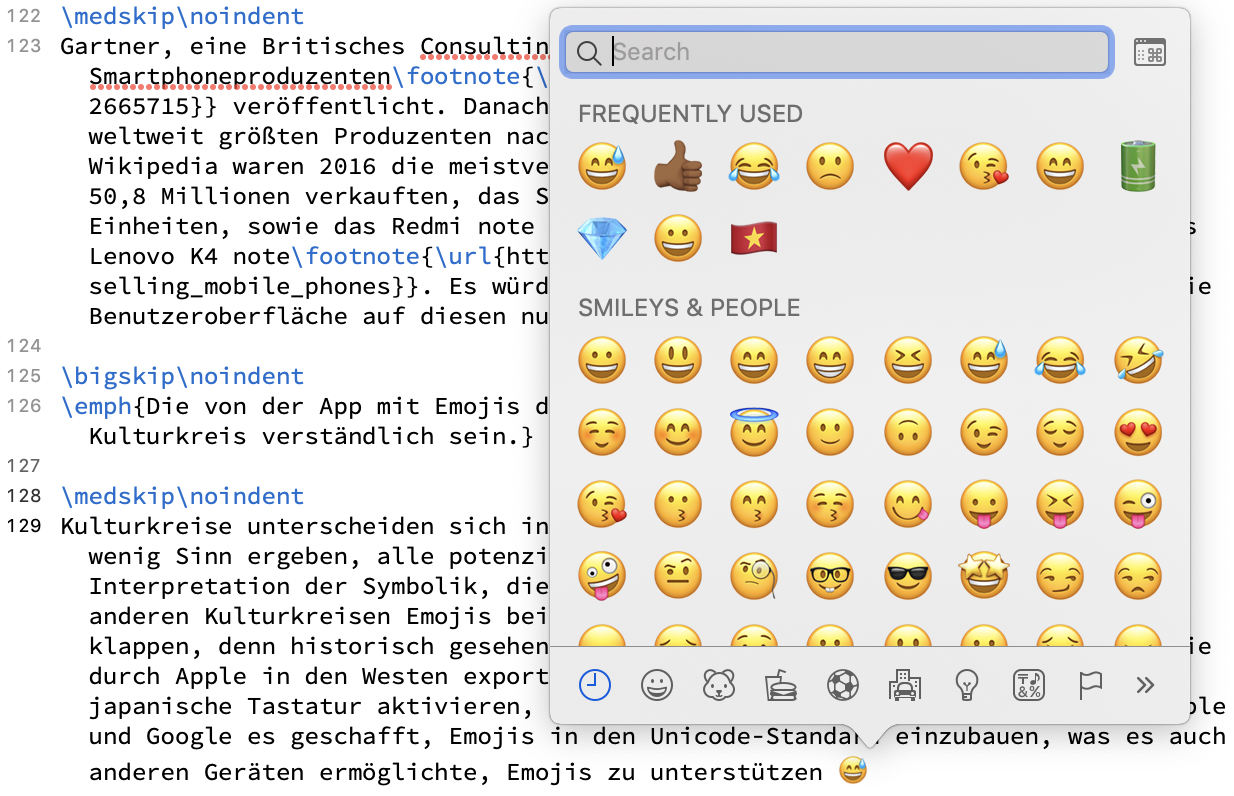
\includegraphics[width=0.75\linewidth]{emojis}
\caption{Emojis auf einem macOS-System}
\label{fig:emojis}
\end{figure}

Möchte man dennoch sicher sein, dass eine reibungslose Kommunikation zwischen unterschiedlichen Kulturen möglich ist, so könnte man stichprobenartig User nach der Bedeutung verschiedener Emojis abfragen, und somit erfassen, ob es Diskrepanzen gibt. Sollten Unterschiede festgestellt werden, so kann man versuchen, die Symbole anzupassen, so dass sie von maximal vielen Kulturen richtig erkannt werden, oder unterschiedlichen Kulturen unterschiedliche Symbole anzeigen. 

\section*{Problem 4: Taxonomie}

\emph{Betrachten Sie die in der Vorlesung vorgestellte Taxonomie von Typen nicht-funktionaler Anforderungen.}

\medskip\noindent
\emph{Klassifizieren Sie die Anforderungen aus Problem 2 gemäß der Taxonomie.}

\bigskip\noindent
\emph{Geben Sie für jede Kategorie der dritten Ebene der Taxonomie (also bspw. Efficiency Requirements, Delivery Requirements) jeweils eine überprüfbare nicht-funktionale Anforderung an. Der Kontext sei der einer Applikation für (Straßen)Karten und Routenplanung. Für die bereits in Teilaufgabe a) verwendeten Kategorien müssen Sie keine weitere Anforderung angeben.}

\end{document}